\documentclass{beamer}
\usepackage[utf8]{inputenc}
\usepackage[francais]{babel}
\usepackage[T1]{fontenc}
\usepackage{amsmath}
\usepackage{amsfonts}
\usepackage{amssymb}
\usepackage{graphicx}
\usepackage{tikz}
\usetikzlibrary{arrows}
\usepackage[squaren,Gray]{SIunits} % Physical units rendering
\usepackage{sistyle}
\usepackage[autolanguage]{numprint}
%\usepackage{xfrac}
\usepackage{bm}
\usepackage{color} % Colors in text
\usepackage[version=3]{mhchem} % Chemical reactions
\usetheme{CambridgeUS}
\setbeamercolor{title}{bg=red!65!black,fg=white}

\setbeamertemplate{sidebar right}
{
  \vfill%
  \llap{\insertlogo\hskip0.1cm}%
  \vskip2pt%
  \llap{\href{http://tex.stackexchange.com/}{A link to tex.sx}\hskip0.2cm}% NEW
  \vskip3pt% NEW
  \llap{\usebeamertemplate***{navigation symbols}\hskip0.1cm}%
  \vskip2pt%
}

\begin{document}

\title{Synthèse de l'ammoniac}
\author{Groupe 1254}
\institute[UCL]{Ecole polytechnique de Louvain-la-neuve}
\date{}
\maketitle
%==========================================================
\begin{frame}{Flowsheet}

\begin{center}
\resizebox{6cm}{6cm}{
	\newpage
\section{Flowsheet}\label{appendix:flowsheet}

\tikzstyle{decision} = [diamond, draw, fill=blue!20,
    text width=4.5em, text badly centered, node distance=3cm, inner sep=0pt]
\tikzstyle{block} = [rectangle, draw, fill=blue!20,
    text width=14em, text centered, rounded corners, minimum height=4em, minimum width=15em, node distance=3cm]
\tikzstyle{block2} = [rectangle, draw, fill=red!20,
    text width=14em, text centered, rounded corners, minimum height=4em, minimum width=15em, node distance=3cm]
\tikzstyle{line} = [draw, -latex']
\tikzstyle{cloud} = [draw, ellipse,fill=red!20, node distance=3cm,
    minimum height=2em]

\begin{center}
	%\begin{tikzpicture}[thick,scale=0.6, every node/.style={scale=0.6}]
	\begin{tikzpicture}[node distance = 3cm, auto]
	    % Place nodes
	    \node [block] (RefPrim) {\textbf{Réformage primaire}(Réformage à vapeur de \ce{CH_4}) $$\ce{CH_4 + H_2O <=> CO + 3H_2}$$ $$\ce{CO + H2O <=> H2 + CO2}$$ \textit{Equilibre à T (sortie)} };
	    \node [block2, left of=RefPrim, node distance=7cm] (Four) {\textbf{Four} \\ Combustion de \ce{CH_4} \\ \textit{Irreversible et complète}};
	    \node [block, below of=RefPrim, node distance=3.5cm] (RefSec) {\textbf{Réformage secondaire} $$\ce{2CH4 + O2 -> 2CO + 4H2}$$ \textit{Considérée comme irréversible et complète à la fin.}};
	    \node [block, below of=RefSec, node distance=3.5cm] (Reacteur) {\textbf{Réacteurs Water-Gas-Shift} $$\ce{CO + H2O -> CO2 + H2}$$ \textit{Considérée comme complète à la fin.} };
	    \node [block, below of=Reacteur, node distance=3.5cm] (AbsComp) {\textbf{Absorption de \ce{CO2} et compression} (séparation d'\ce{H2 O}) \\ \textit{Considérées complètes.}};
	    \node [block, below of=AbsComp, node distance=3.5cm] (Synth) {\textbf{Synthèse d'\ce{NH3} et séparation} $$\ce{N2 + 3H2 <=> 2NH3}$$ \textit{Considérées complètes.}};
	    \node [right of =AbsComp, node distance=6cm] (nothing1){};
	    \node [below of =Synth] (nothing2){};
	    \node [left of =RefSec, node distance=6cm] (nothing3){};
	    \node [above of =RefPrim, node distance=4cm] (nothing4){};
	    \node [left of =Four, node distance=5cm] (nothing5){};
	    \node [above of =Four, node distance=4cm] (nothing6){};
	    % Draw edges
	    \path [line] (RefPrim) -- node {\ce{CH4}, \ce{H2O}}(RefSec);
	    \path [line] (Four) -- node {ENERGY} (RefPrim);
	    \path [line] (RefSec) -- (Reacteur);
	    \path [line] (Reacteur) -- node {\ce{CO2(g) + H2(g)}} (AbsComp);
	    \path [line] (AbsComp) -- (Synth);
	    \path [line] (AbsComp) -- node {\ce{CO2(g)}, \ce{H2O(g)}}(nothing1);
	    \path [line] (Synth) -- node {\ce{NH3(l)}, \ce{Ar(g)}}(nothing2);
	    \path [line] (nothing3) -- node {\ce{O2(g)}, \ce{N2(g)},\ce{Ar(g)}}(RefSec);
	    \path [line] (nothing4) -- node {\ce{CH4(g)}, \ce{H2 O(l)}}(RefPrim);
	    \path [line] (Four) -- node {\ce{CO2+2H2O}} (nothing5);
	    \path [line] (nothing6) -- node {\ce{CH4(g), H2O(l)}} (Four);
	\end{tikzpicture}
\end{center}
}
\end{center}
\end{frame}

\begin{frame}{Quid du biogaz comme alternative au méthane pur?}
	\begin{columns}
		\begin{column}{0.40\textwidth}
		Composition:
			\begin{itemize}
			\item 50 à \unit{70}{\%} de \ce{CH4}
			\item 15 à \unit{45}{\%} de \ce{CO2}
			\item  \unit{5}{\%} de \ce{H2O}
			\item 0 à \unit{2}{\%} de \ce{H2S}
			\item impuretés (négligeable)
			\end{itemize}
		\end{column}
		\begin{column}{0.40\textwidth}
		Avantages:
			\begin{itemize}
			\item Ecologique 
				\begin{itemize}
				\item \ce{CO2}
				\item \ce{CH4}
				\end{itemize}
			\item Réduction des problèmes liés au transport
			\item Réduction de la consommation d'énergie
			\end{itemize}
		\end{column}
	\end{columns}
\end{frame}
\begin{frame}{Faisabilité}
	\begin{columns}
		\begin{column}{0.40\textwidth}
		\begin{itemize}
		\item \unit{1500}{t/j} de \ce{NH3} $\Longrightarrow$ \unit{1509188}{m^3} de biogaz
		\item Région wallonne : 86.6 millions de \cubic\meter \ de biogaz annuellement (potentiel)
		\item Impossibilité de remplacer le \ce{CH4} totalement par du biogaz
		\end{itemize}
		\end{column}
		\begin{column}{0.40\textwidth}
		\begin{figure}
		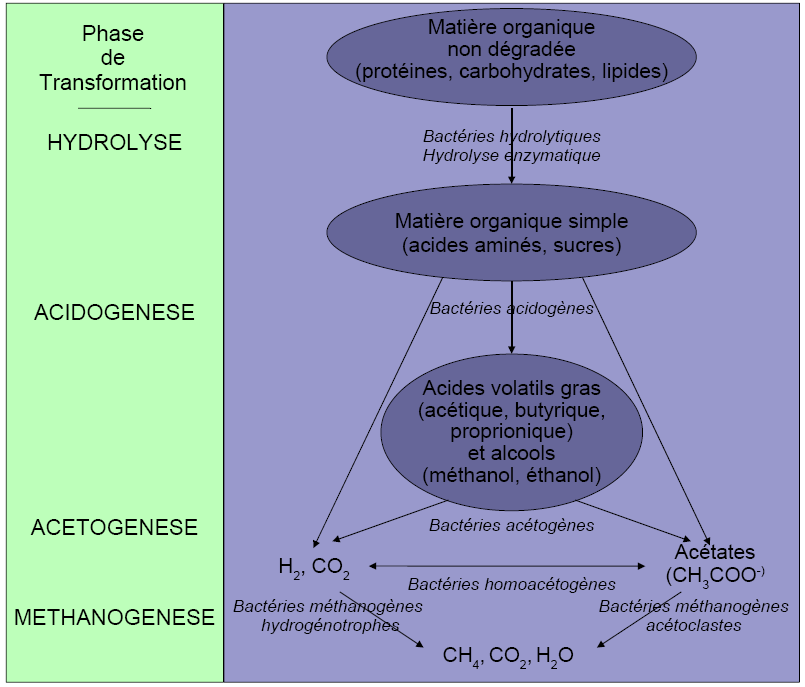
\includegraphics[scale=0.2]{schema/process_biologique_methanisation_et_biogaz.png}
		\end{figure}
		
		\end{column}
	\end{columns}
\end{frame}
\end{document}